\subsubsection{Deliveries, Loads and Cooperative Results}
Delivery belongs to one campaign and has one associated TransportRecord, with a
registered Worker driver. OliveBatch stores one actual source property and optional
parcel, with known source quantities separate from official ticket weights.
TransportRecord may retain a transport-document reference and declared origin;
these do not allocate a mixed load or make parcels mandatory.
Figure~\ref{fig:er-deliveries} shows the delivery and source-result relationships.
\begin{figure}[!htbp]\centering
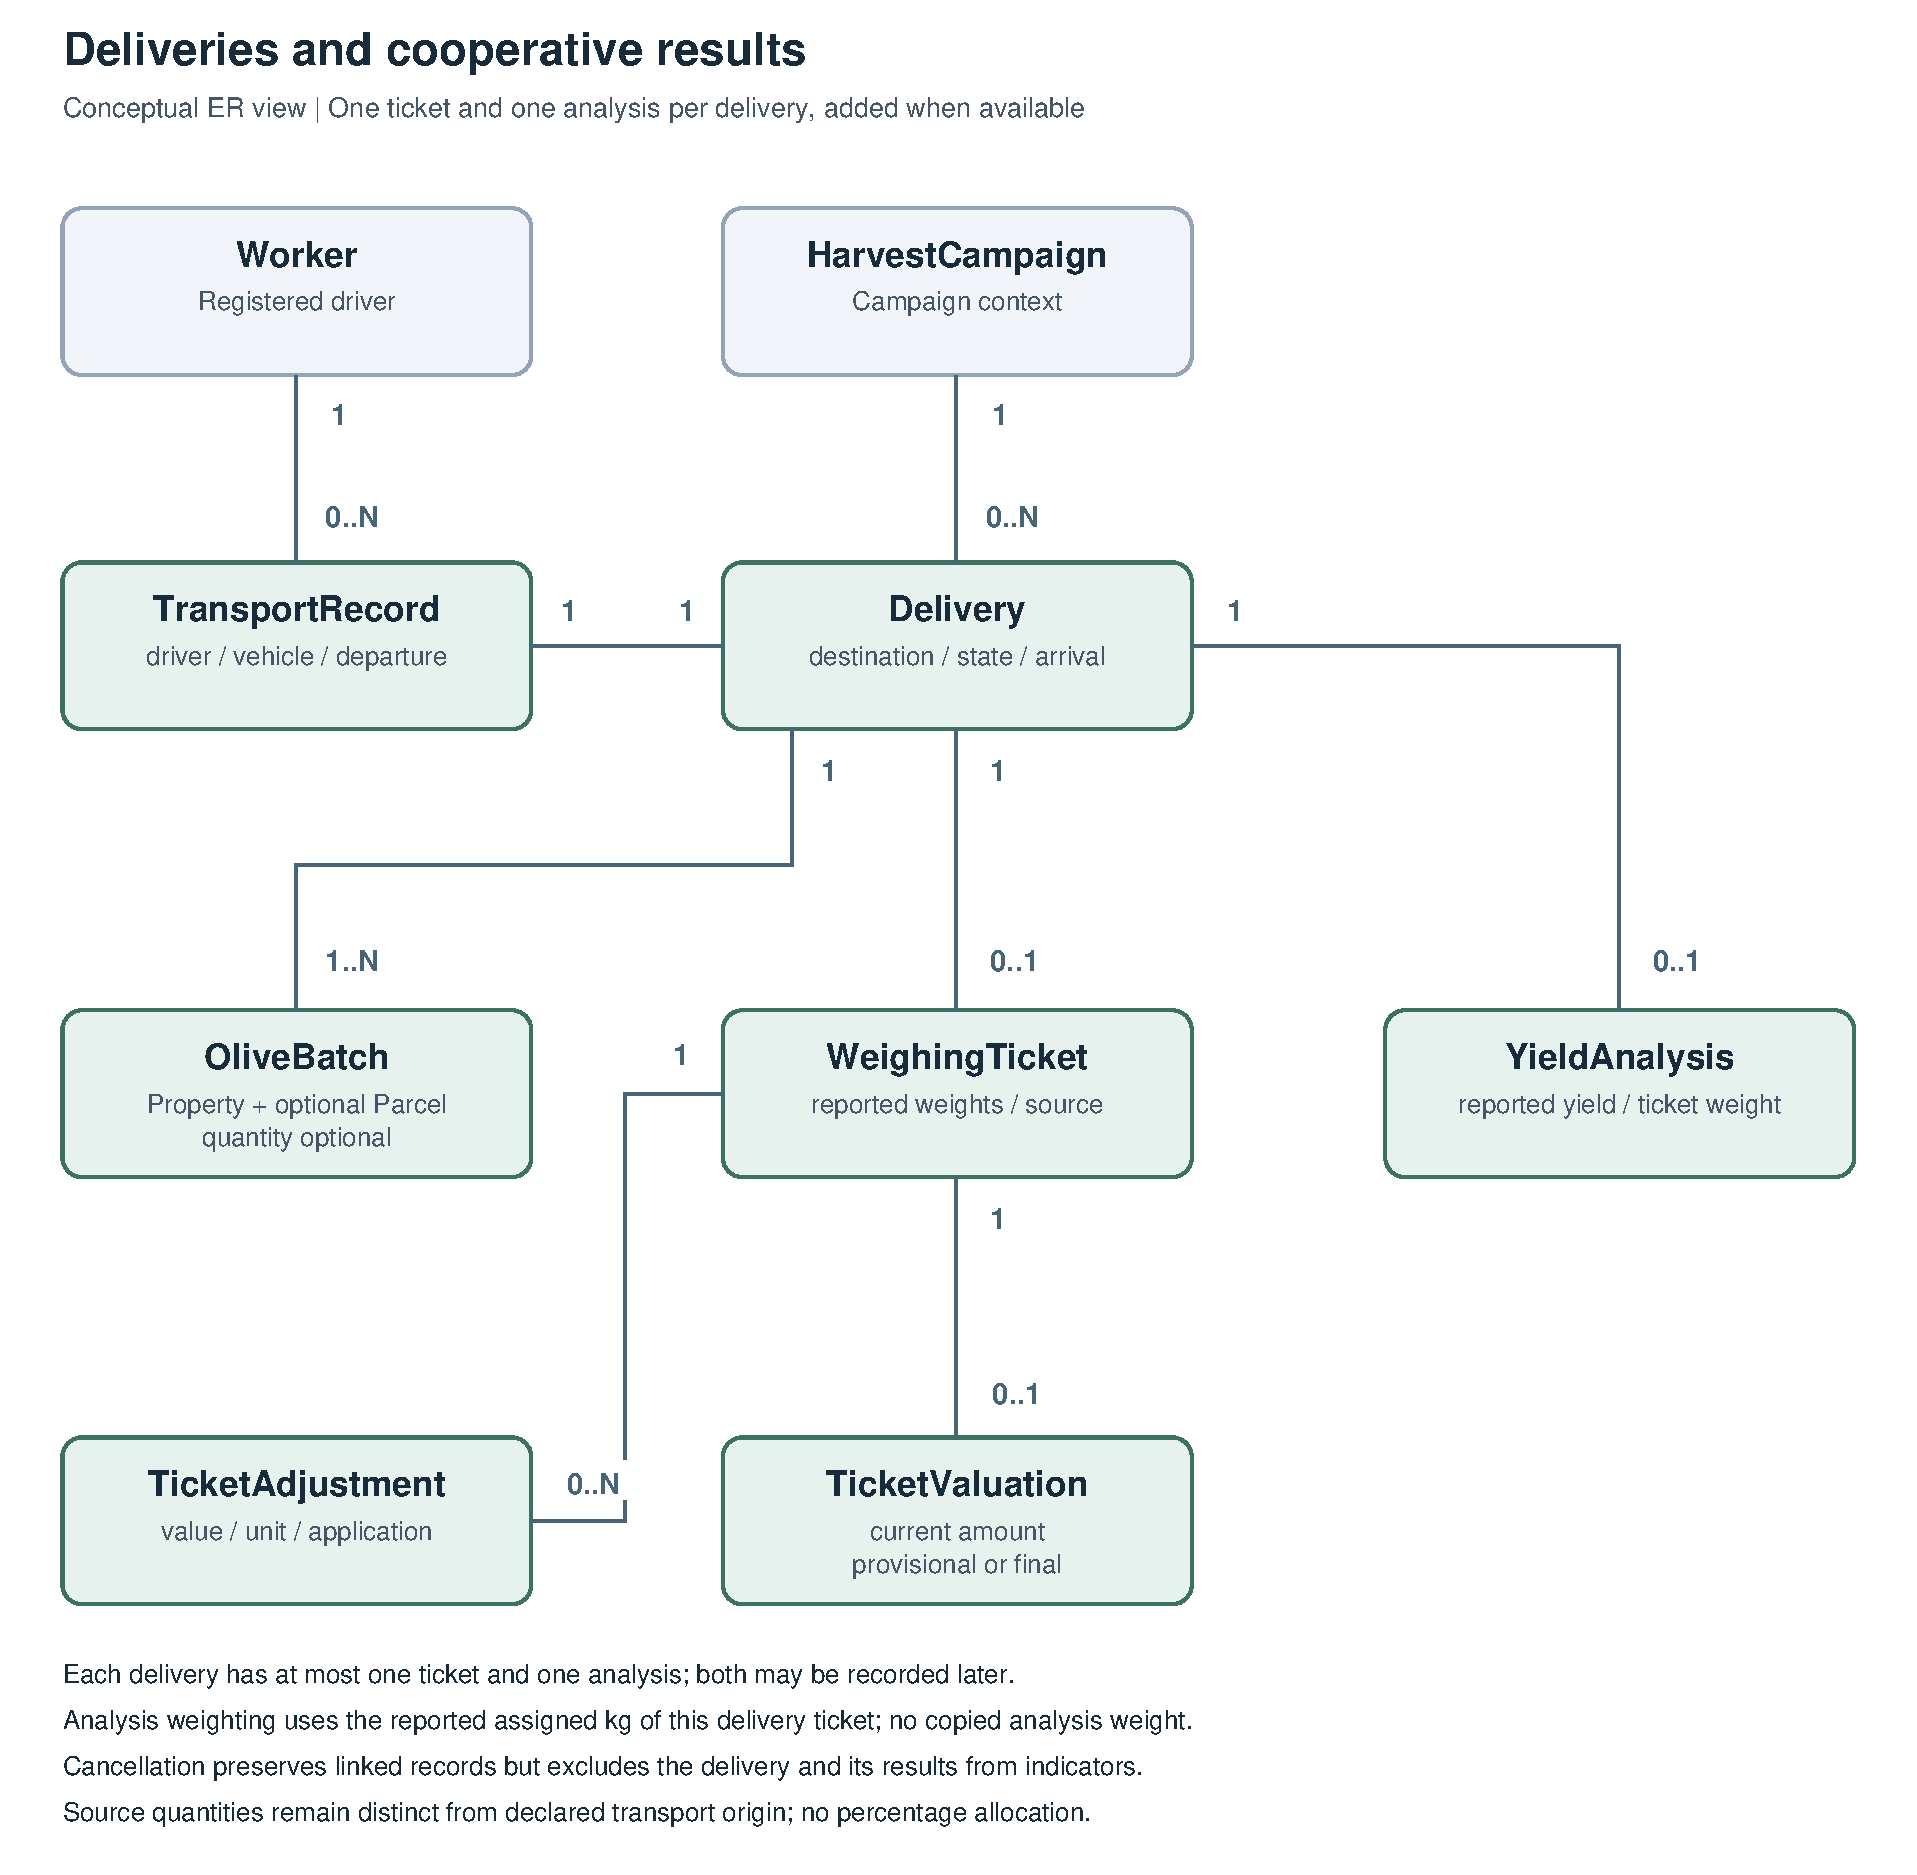
\includegraphics[width=\linewidth]{er-deliveries.pdf}
\caption{Each delivery has at most one ticket and one analysis. Source batches remain distinct from official weights.}
\label{fig:er-deliveries}
\end{figure}
WeighingTicket has a unique delivery reference and an optional canonical reported
accepted assigned weight in kg. Other weights retain source meanings/units. Optional
weighing start/end and reported excess duration are descriptive source facts.
TicketAdjustment also represents reported monetary penalties, protected by financial
grants; the application does not calculate or reapply them.
YieldAnalysis has a unique delivery reference and the reported yield percentage.
Its weighting reference is reached through the delivery's ticket; no independently
editable reference-weight copy is stored. TicketValuation is one current reported
amount per ticket. SourceAttachment supplies separate evidence links.
Source records may exist while Delivery is In transport. Indicator queries use
the Delivered, non-cancelled parent predicate in \hyperref[br:038]{\identifier{BR-038}}; source
existence alone does not confirm receipt.
The current model records known quantities in OliveBatch and one total amount
in TicketValuation; it has no field for monetary amounts by source. Mixed-load
amounts therefore remain unallocated by property/parcel, even when source quantities
are known. Supporting reported source amounts would require an explicit model
extension and review. No monetary allocation proportional to weight is inferred.
Delivery cancellation stores reason, time and actor while preserving dependent
records; lifecycle and correction behaviour follow \hyperref[br:031]{\identifier{BR-031}}.
Eligible hard deletion removes composed TransportRecord and OliveBatch rows in the
same validated operation, only when no ticket, analysis, valuation or evidence blocks it.

\paragraph{Ticket source fields.}
A validated source metadata snapshot holds source date/season, line, sample/member
references, quality/variety, municipality, literal POL/PAR/REC/PARAJE and locator
(Table~\ref{tab:source-ticket}). These source facts do not silently edit properties,
parcels, worker identities or transport records. Total kg and other source weights use validated reported-weight entries; KILOS ASIGNADOS uses only the typed canonical assigned kg field, which remains unknown if no accepted weight was reported. MEDIANERIA records the accepted percentage without generating a second assigned-weight value. Store printed
duration in seconds separately from start/end and excess time, with discrepancies
flagged for review. No penalty-calculation entity or integration is introduced.
